\newcommand{\definice}{\paragraph{Definice.}}

\chapter{Compilation and optimization}

In the beginning of this chapter, we will look into the composition of modern
programs, their codebase size and organization. We will continue with an
overview of compiler's workflow, introduce optimization passses and link-time
optimization framework.

\section{Code organization and codebase size}

Let us start by examining some of the code bases for programs we use every day.
A lot of developers run Linux, Firefox (or other browser) and GCC every day, but
unless we're developing one of them, we don't really have a good idea of how large
they are. It is not hard to guess they are enormous, containing millions of
lines of code. But how many exactly, and how is the number growing?
The chart in Figure \ref{figure-loc} show historical development over the past
10 years.

\begin{figure}[h!]
\label{figure-loc}
\centering
	\hspace{-1cm}\includegraphics{graphs/loc/loc.pdf}
\caption{Codebase size of Firefox, Chrome and GCC over time. [Data provided by
	openhub.net]}
\end{figure}

It might be tempting to say that the code will be split into many libraries. It
is no secret that for example Firefox bundles many libraries inside, they might
be compiled separately, resulting in many self-contained libraries in the
distribution. Figure \ref{figure-firefox-objsize} shows 8 largest libraries
contained in a standard Firefox distribution. The main library is 66.39 MB
large, the second largest is only 1.51 MB. This is due to speed optimizations,
as the developers noticed a significant start-up delay if all libraries are
loaded separately, and bundled them together into a single library. This also
means that compiler optimizing this library has to deal with all the code at
included.

\begin{figure}[h!]
\label{figure-firefox-objsize}
\centering
\includegraphics[angle=-90,trim=0 30 10 0,clip]{graphs/firefox-objsize/objsize.pdf}
\caption{Firefox 50.0.2 object sizes by binary}
\end{figure}

We should keep these numbers in mind while writing a compiler.

\section{Program compilation}

Only the simplest programs consist of a single source file, many programs have
tens, hundreds or even thousands of source files. This not only serves an
organizational purpose, but also allows the programmer to choose different
optimization flags for different files, or even write different parts in
different languages. A mechanism called {\sl separate compilation} is used to
compile and combine (link) all of them together, to form a finished program.
Figure \ref{figure-non-lto-workflow} shows the transformation using standard GCC
and Binutils (compiler and linker).

First step is to compile every  source file into object file. In this phase, a
compiler is invoked and does all the work necessary to convert source code into
binary, including code generation. The result is stored in an object file,
including required metadata, for example symbol table. This step is independedt
for each source file, so they can be processed in parallel. 

Second step consists of simple linking. A linker inspects all generated objects,
resolves required and provided symbols, dynamic libraris, and produces a
final executable. The linker usually doesn't modify code in object files, as it
only understands symbols and sections.

\begin{figure}[h!]
\label{figure-non-lto-workflow}
\centering
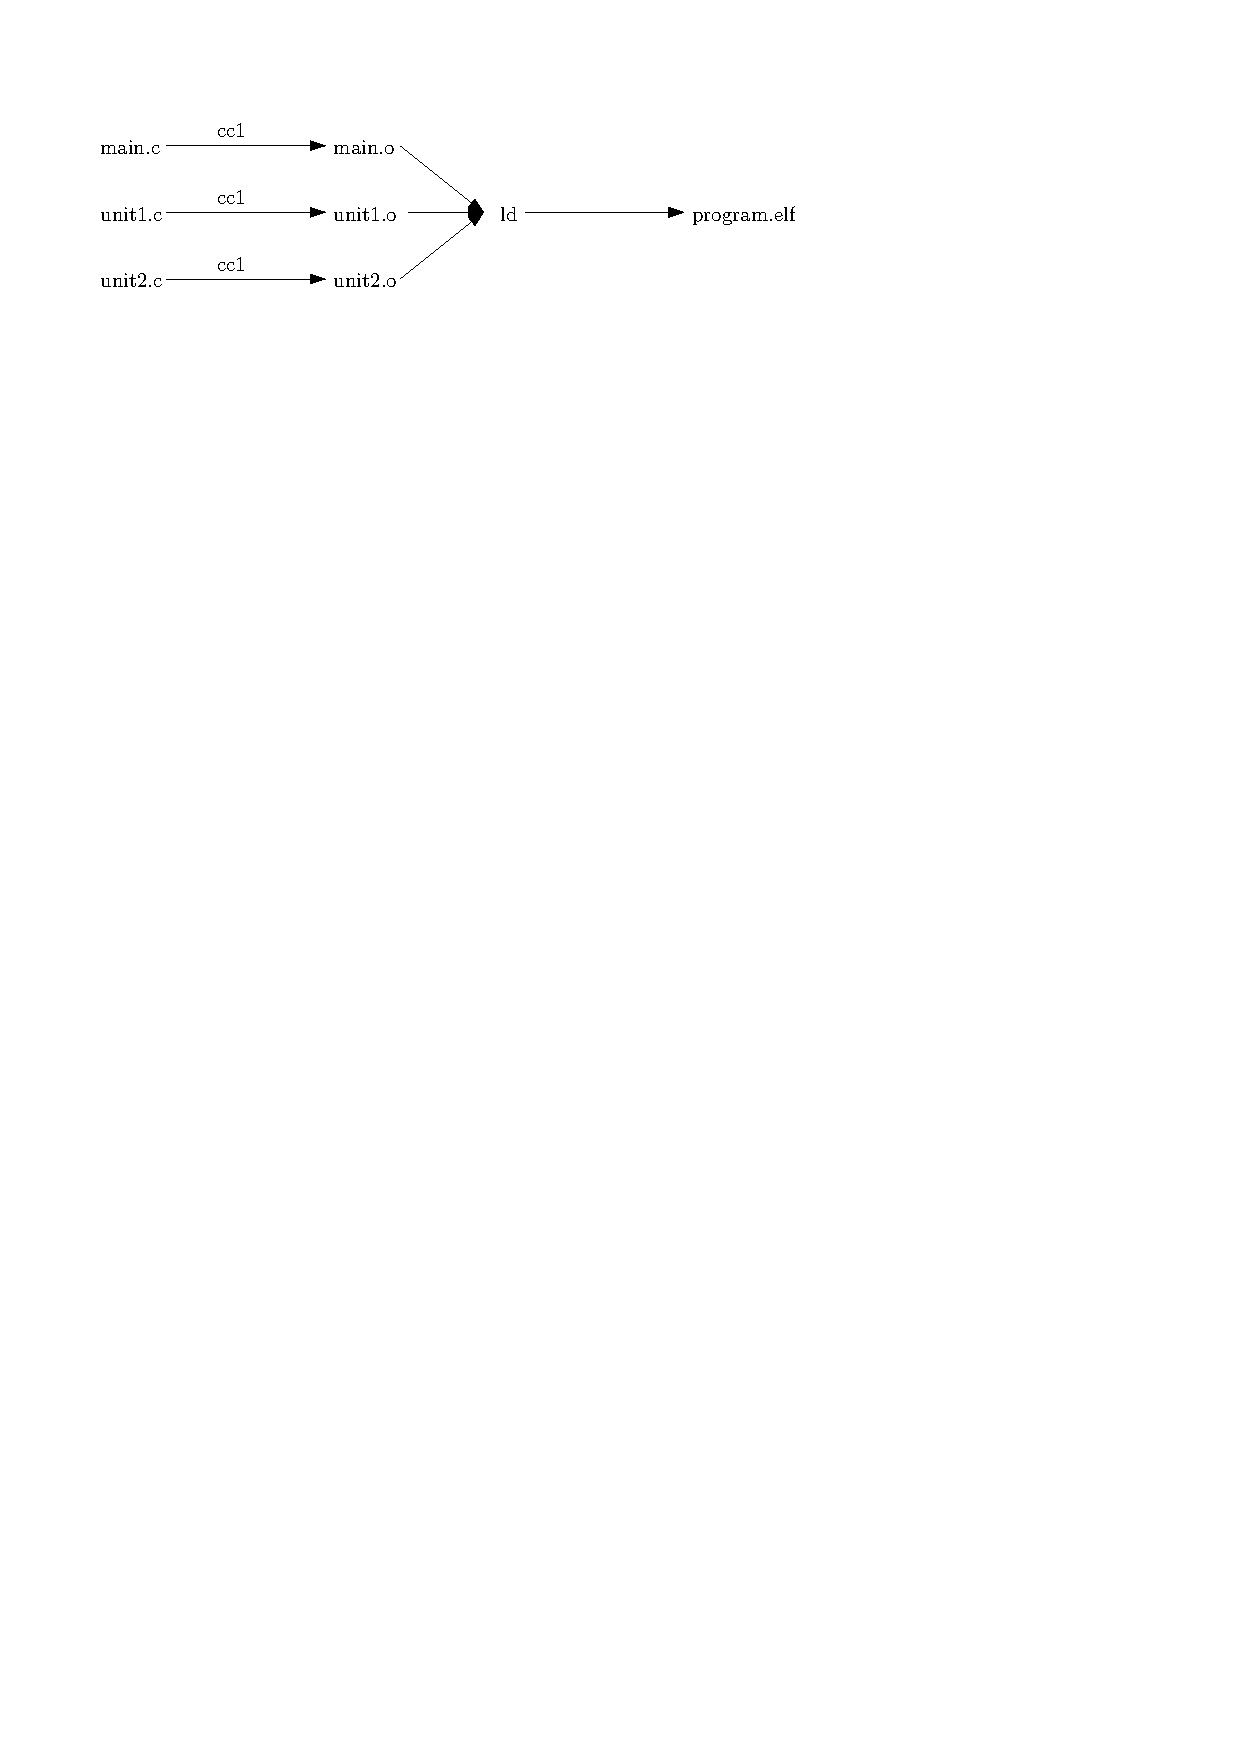
\includegraphics{./img/non-lto-workflow.pdf}
\caption{Standard workflow for separate compilation}
\end{figure}


\section{Compilation phases}

To compile a program written in high-level programming language into a machine
code requires many steps. To make orientation easy, and to support code
re-usability, a compiler usually consists of these three parts:

\paragraph{Front End} understands the input language, builts abstract syntax
tree and converts in into a common intermedialy language (IL) to all front ends
and the middle end.

\paragraph{Middle End} analyses the IL code and does most highlevel
optimizations. This includes splitting the code into basic blocks, building a
Control Flow Graph (CFG), dead code elimination, constant propagation, profile
driven transformations and many others \TODO{Ref forward.}

\paragraph{Back End} converts IL code into machine code, optimizing on the
lowest level, being able to schedule individual instructions and registers.

During this process multiple intermediary languages are used, sometimes more at
the same time (usually during transition to the lower-level language).

\begin{description}
	\item[GENERIC] is the highest-level IL used by the Front End, able to
		represent syntax trees and language-specific features.
	\item[GIMPLE] is tuple-based IL language, able to represent only simple
		expressions common to all languages. It is unable to represent many
		high-level constructs as for example loops.
	\item[RTL] (Register Transfer Language) is a low level language similar to
		machine code, containing algebraicly described instructions, as should
		be generated.
\end{description}


\section{Link-time optimization}

The idea of interprocedural and link-time optimization (LTO) is old. One of the
first ideas were published in 1970s \cite{Allen1974}, \cite{Allen1976}. It was
already supported in MIPSPro in 1990s\TODO{CITE}, which was later released in 2000 as
Open64 under GNU GPL. The compiler suite LLVM supports link-time optimization by
design, from their first release in 2002 \cite{lattner2002llvm}.  GCC was late
with their link-time optimization framework was proposed in 2005 [Ref:DraftLTO],
[REF:DraftWHOPR] and released in 2009.

Programs are usually compiled separately, meaning every source file is compiled
into it's own object file. All the object files are then linked together,
forming the final binary. This is a good technique, as it not only allows
logical grouping of code into files, but also change in one file does not force
recompilation of all other files. On the other hand, it also means that
optimizer only sees one file at a time, and some optimizations might be hard or
even impossible to do.  One example might be devirtualization in C++. As the
class it's descendants are usually in a separate file, the compiler has no way
of knowing that there is only one possible virtual method, and devirtualize it.
This often happens when using Mock objects\footnote{Objects that mimic some
behavior, for example a piece of hardware} for testing.

Some authors worked around this limitation. For example SQLite or older versions
of KDE support code concatenation in their build system. This results in one
huge source file being passed to the compiler. The result was good in it's day,
but still has some issues. All the code needs to be parsed at once, which
increases memory usage and does not scale well, as language parsers are not
usually parallel, and thus cannot make use of multi processor system.

\begin{figure}[h!]
	\label{figure-lto-workflow}
	\centering
	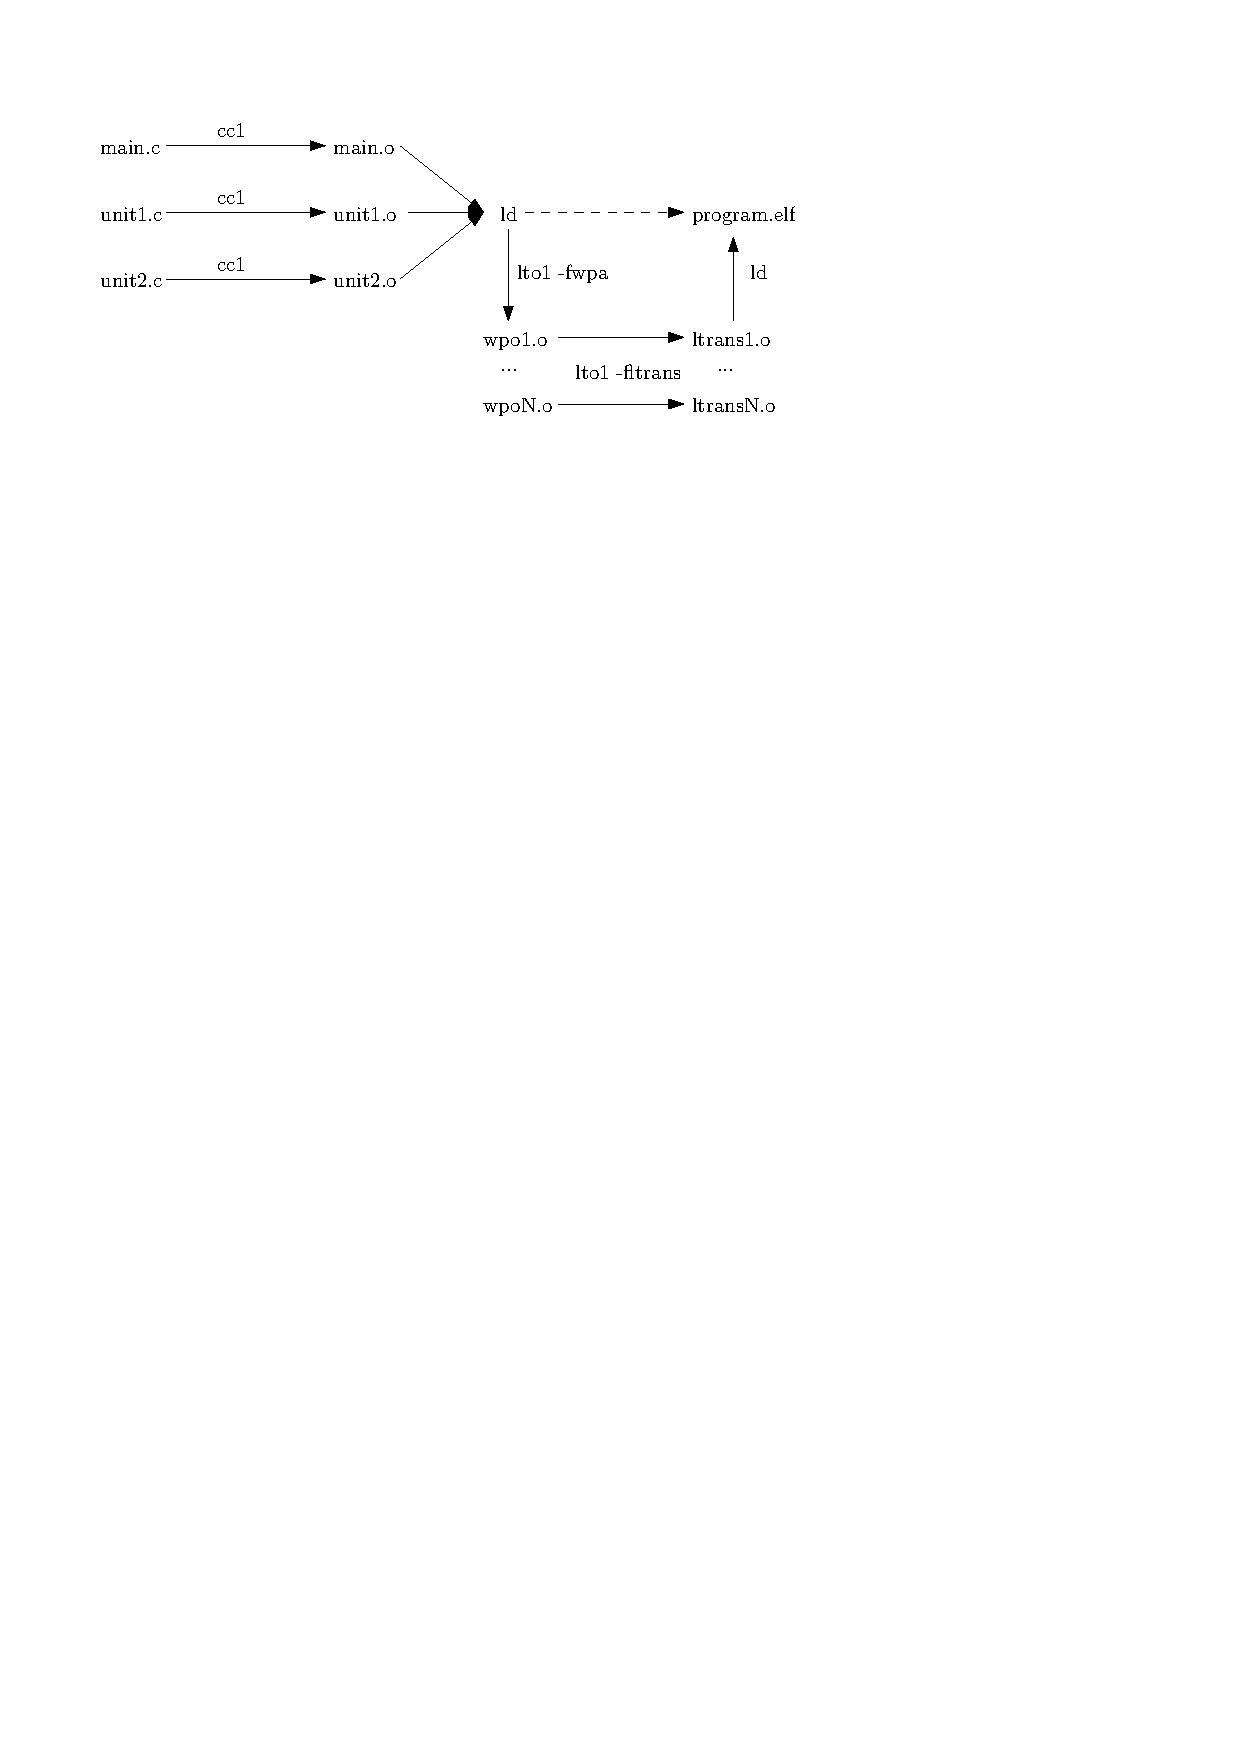
\includegraphics{./img/lto-workflow.pdf}
	\caption{Compiling source code into binary}
\end{figure}

The LTO framework (see Figure \ref{figure-lto-workflow}) solves these problems by keeping separate compilation, but
instead of generating classical object files containing machine code, the
middle end stops and writes GIMPLE representation into the object, including
some metadata (for example the call graph).

Instead of generating library, the linker then picks up the GIMPLE
representation and invokes the compiler again. GCC was designed to perform most
of the optimizations in parallel, and the process has been further split into
two stages. The sequential WPA (Whole Program Analysis) stage and parallel
LTRANS (Local TRANSformations) stage.

\paragraph{WPA} stage performs declaration and type linking, and decision stage
of interprodecural optimizations. It ends by partitioning the code into smaller
pieces called {\sl LTO partitions}. The partitioning happens with regard to the
code being optimized, for example to minimize cross-partition edges.

\paragraph{LTRANS} stage then performs optimizations decided by WPA stage,
followed by local optimizations and code generation.


\section{Evaluating GCC performance}

As we previously noted, we will be focusing on the GCC compiler suite. In this
section, we will cover the experimental setup, evaluate compile time in a few
programs and extract practical information on resources needed and
anticipated use.

We will publish source code used to take these measurements, so anyone can
reproduce these results, and perhaps use for comparison on his/her own work.We 
will also omit some technical details in this chapter, but will include them in
the Appendix \TODO{link}.

\subsection{Compiler}

For further measurements, we will be using GCC compiled from branch {\tt
gcc-5-branch} (via github.com mirror, but any up to date repository will
suffice). The reason for this branch is simple: it's relatively fresh branch,
that supports most of the latest features, but will not change during
development and provide stable base for testing, while still receiving bug fixes
for the time being. Most of the benchmarking is non-intrusive but some involve
large data dumps which may slow us down. This will be noted whenever appliccable.


\subsection{Software under test}

Many opensource programs are available for testing, however a good candidate has
to fulfill a few requirements to make testing straightforward and reproducible.

\begin{itemize}
	\item Written in C++ (preferred) or C.
	\item A good compatibility with current GCC versions (5.x and 6.x)
	\item Flexible and robust build system.
	\item Mid to large codebase.
	\item Preferably monolithic binary.
\end{itemize}

It is surprisingly difficult to find projects that fit all of those
requirements. Many popular programs were ruled out immediately. For example the
build systems of MySQL and Inkscape is very inflexible and has trouble with LTO
compilation. GIMP consists of many plugins which doesn't pose any challenge for
the current link-time optimizer. However, a few others passed:

\paragraph{Firefox} was an easy choice, as it is an established benchmark for GCC
and though there were a few issues in the beginning, later versions are polished
and fullfill all the requirements. There is only one problem, and that is it
takes approximately 25-36 hours to compile firefox with non-modified GCC
sources, which isn't very good for development. The main reason for this
slowdown is excessive RAM usage, which doesn't allow parallel LTO pass.  
The specific version used in testing is {\it Firefox 48}.

\paragraph{Merkaartor} is an OpenStreetMap editor written in C++ with medium
sized code-base. It utilizes Qt framework, a lot of C++ constructs and links
plenty of objects into a single binary, and uses a lot of C++ constructs.

\paragraph{SQLite} is a SQL database engine in a single source file with a
medium (to small) sized code-base. It offers fast compilation times 

The specific version used in testing is {\it Merkaartor 0.18.3-rc1}

\subsection{Other software and hardware}

\subsubsection{Hardware}

Where relevant, the following machine was used for testing:

\begin{itemize}
	\item Intel Xeon E3-1231-v3 @ 3.40GHz (Haswell)
	\item 32GB DDR3 RAM @ 1600MHz, consisting of 4 modules KHX1600C10D3/8G
	\item 120GB Intel 520 SSD, SSDSC2CW120A3
\end{itemize}

I consider this setup to be high-end for desktop computing, and much more than
should be required. Other machines were used during testing, but all time
results will be quoted for the one above.

\subsubsection{Software}

The system was running 64bit Linux kernel 4.5 and standard Gentoo Linux
installation. 

Memory and cpu usage measurements were taken using Linux Control Groups for
whole compilation process, including GNU make and other tools. The data were
sampled at 1 second intervals, which is more than enough. Total CPU usage is
known precisely, as control groups keep cumulative counter. The activity at a
given point is used only as a pointer as to how many cores are currently
computing. As for the memory, the second interval is fine as well, as we are not
allocating and freeing memory rapidly. In fact, most of our allocations will be
done at the beginning of an analysis.

\begin{figure}[h!]
	\label{figure-firefox-ipa-kpta}
	\centering
	\includegraphics{./graphs/firefox-ipa-kpta/firefox-ipa-kpta.pdf}
	\caption{Building libxul.so with {\tt -fipa-kpta -flto=8}}
\end{figure}
